\documentclass{article}

\usepackage{graphicx}

\usepackage[utf8]{inputenc}
\usepackage[T1]{fontenc}
\usepackage[danish,english]{babel}

\usepackage{footnote}
\usepackage{listings}
\usepackage{lastpage}
\usepackage{fancyhdr}

\usepackage{amssymb}
\usepackage{amsthm}
\usepackage{amsmath}
\usepackage{latexsym}
\usepackage{enumerate}
\usepackage{subfigure}

\usepackage[T1]{fontenc}
\usepackage{lmodern}
\usepackage{vaucanson-g}
\usepackage{multido}

\newtheoremstyle{dotless}{}{}{\itshape}{}{\bfseries}{}{ }{}
\newtheoremstyle{itless}{}{}{}{}{\bfseries}{}{ }{}

\theoremstyle{dotless}

\newcounter{maj}
\newcounter{min}

\renewcommand{\thesection}{}
\newcommand{\Section}[1]{\section{#1}
\setcounter{min}{1}}

\renewcommand{\thesubsection}{}

\pagestyle{fancy}
\lhead{Machine Learning, A-1}
\rhead{Morten Winther Olsson, hkv518}
\cfoot{\thepage\ of \pageref{LastPage}}

\title{\begin{tabular}{c}
Statistical Methods\\
for\\
Machine Learning\\
Assignment 1\\
\end{tabular}}
\date{18. February 2014}
%% \date{\today}
\author{\begin{tabular}{c}
Kristina  Aluzaite (ljg630)\\
Mads Ølsgaard (gtw631)\\
Morten Winther Olsson (hkv518)\\
\end{tabular}}

\begin{document}

%% \markboth{Im So Meta Even This Acronym}{Reelect your Teddy Bear}

\maketitle
\thispagestyle{fancy}

\newpage{}

%% \tableofcontents{}

%% \newpage{}

\Section{Introduction}


\Section{II.1 Classification}

\subsection{II.1.1 Linear discriminant analysis \& II.1.2 LDA and normalization}

%% \subsection{II.1.2 LDA and normalization}

For the LDA we are using the mlpy implementation because an error in our own implementation caused all data points to be classified to all classes.\\

Error rate is simply calculated as 1 minus number of correct classifications over total datapoints. See table \ref{result1.1}\\

\begin{table}[h]
\label{result1.1}
    \centering
    \begin{tabular}{l| r}
        Label & error \\ \hline
        Non-normalized, test & 0.2105 \\
        Non-normalized, train & 0.14 \\ \hline
        Normalized, test & 0.2105 \\
        Normalized, train & 0.14
    \end{tabular}
\caption{Results of Iris classification}
\end{table}

Given that the model is fitted around the training data, it is no surprise that the training data has a lower error rate than when testing on the test set.

We see no change in normalizing the data. This is because LDA assumes all classes to be normally distributed and with the same covariance. So normalizing data won't affect the covariance matrix.

\subsection{II.1.3 Bayes optimal classification and probabilistic clas-
sification}

The Bayes Optimal is defined as the classifier that gives the lowest risk.\\

$argmax(v_j\in V)=\sum_{h_i\in H}{p(v_j|h_i)P(h_i|D)}$\\

System that classifies new instances based on the equation above are called Bayes Optimal Classifiers.

In our case, the hypothesis set $H=\{h_1, h_2\}$, where $h_1=0$, $h_2=1$, and $P(h_1)=0.25$, while $P(h_2)=0.75$.\\

Let $V=\{\bigoplus,\bigodot\}$\\
suppose: $\begin{matrix}\bigoplus\texttt{ if }1\\
\bigodot\texttt{ if }0\end{matrix}$\\

Given the data set D:\\
$P(h_1, D ) = 0.25$\\
$P(h_2, D ) = 0.75$\\

Probabilities of classifying new instances as $\bigoplus$ or $\bigodot$ for the $h_1$ or $h_2$\\
$(\bigodot, h_1) = 1$\\
$(\bigodot, h_2) = 0$\\
$(\bigoplus, h_1) = 0$\\
$(\bigoplus, h_2) = 1$\\

Therefore, multiplying and summing all the the conditionals we get:\\
$\sum_{h_i\in H}{P(\bigoplus|h_i)P(h_i|D)} = 0.75$\\
$\sum_{h_i\in H}{P(\bigodot|h_i)P(h_i|D)} = 0.25$\\

And the most probable classification of the new instance is:\\
$argmax(v_j\in\{\bigoplus,\bigodot\})=\sum_{h_i\in H}{p(\bigoplus|h_i)P(h_i|D)}=\bigoplus$\\

The Bayes risk is defined as a minimum risk over all possible measurable functions H.\\
For the classifier above, the bayes risk is $R=0.25$, as the $P(h_2=0) = 0.25$\\

The risk of the probabilistic classifier given the data is a combination of probabilities of classification for different states. We sum the products of the event probability times the risk of the false prediction.\\

for $h_1 = 0$, the probability of a false prediction is $0.75$ and the hypothesis $h(x) =0$ occurs $0.25$ of the time; and\\
for $h_0 =1$ the probability of a false prediction is $0.25$ and the hypothesis is true $0.75$ of the time.\\

Hence, the risk of the classifier is $0.75*0.25 + 0.25 * 0.75 = 0.375$.\\

\Section{II.2 Regression: Sunspot Prediction}

\subsection{II.2.1 Maximum likelihood solution}

We use a simple linear model for our regression of the sunspot data\\

\begin{equation} \label{simplelinear}
y(\vec{x},\vec{w}) = w_0 + w_1x_1 + ... + w_Dx_D
\end{equation}\\

To facilitate this we set the basis function $\phi_j(x) = x_j$ where \emph{$j$} denotes the $j$'th value in the observation vector $x$. So $j \in \{0 \dots D\}$. For $j = 0$, $1$ is returned. In the code this is facilitated by adding a column of $1$'s to the training and testing data.\\

This gives us the design matrix $\Phi$,\\

\begin{equation} \label{Phi}
\Phi = 
 \begin{pmatrix}
  1 & X_{1,1} & X_{1,2} & \cdots & X_{1,j} \\
  1 & X_{2,1} & X_{2,2} & \cdots & X_{2,j} \\
  \vdots & \vdots  & \vdots  & \ddots & \vdots  \\
  1 & X_{l,1} & X_{l,2} & \cdots & X_{l,j}
 \end{pmatrix}
 \end{equation}\\

Where $l$ is the number of observations.

$\vec{W}$ is found by taking the pseudo inverse of the design matrix using numpy's \texttt{np.linealg.pinv()} function.

Results are tested using the \emph{root mean square} (RMS) error seen in table \ref{result2.1}. Selection 3 yields the lowest error and is therefore the best selection.

This makes good sense, since we know that sunspots follow an 11 year cycle and selection 3 is the only selection that has data from before and after 11 years before any given year.

\begin{table}[h]
\centering
\label{result2.1}
    \begin{tabular}{l| r}
        Selection & RMS \\ \hline
        1 & 35.47 \\
        2 & 28.83 \\
        3 & 18.77
    \end{tabular}
\caption{Results of sun-spot prediction using Maximum likelihood solution}
\end{table}

\begin{figure}[h]
    \centering
    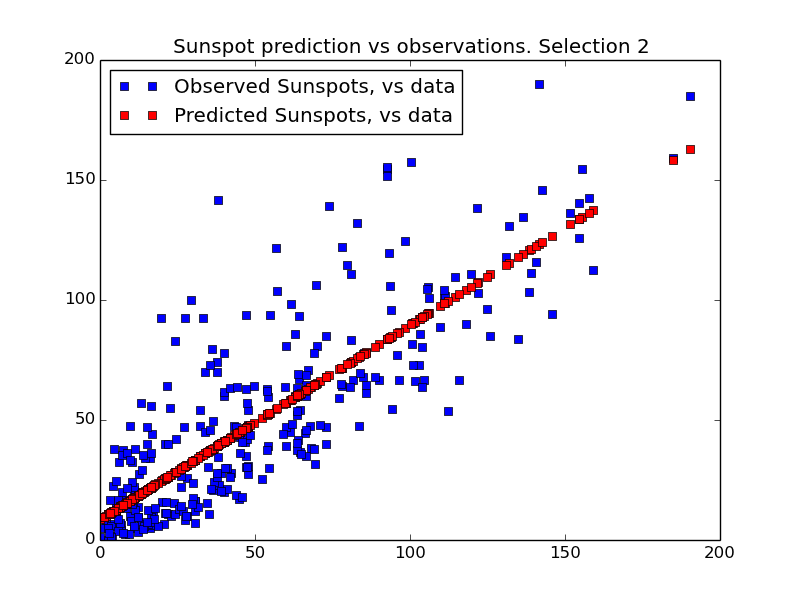
\includegraphics[width=0.5\textwidth]{src/img/predictions_over_obs.png}
    \caption{Showing predictions and actual observations as a function of data from selection 2. We clearly see the linearity of the model, but also that the observations do in fact center around a linear line.}
    \label{fig:pred_obs}
\end{figure}

\begin{figure}[h]
    \centering
    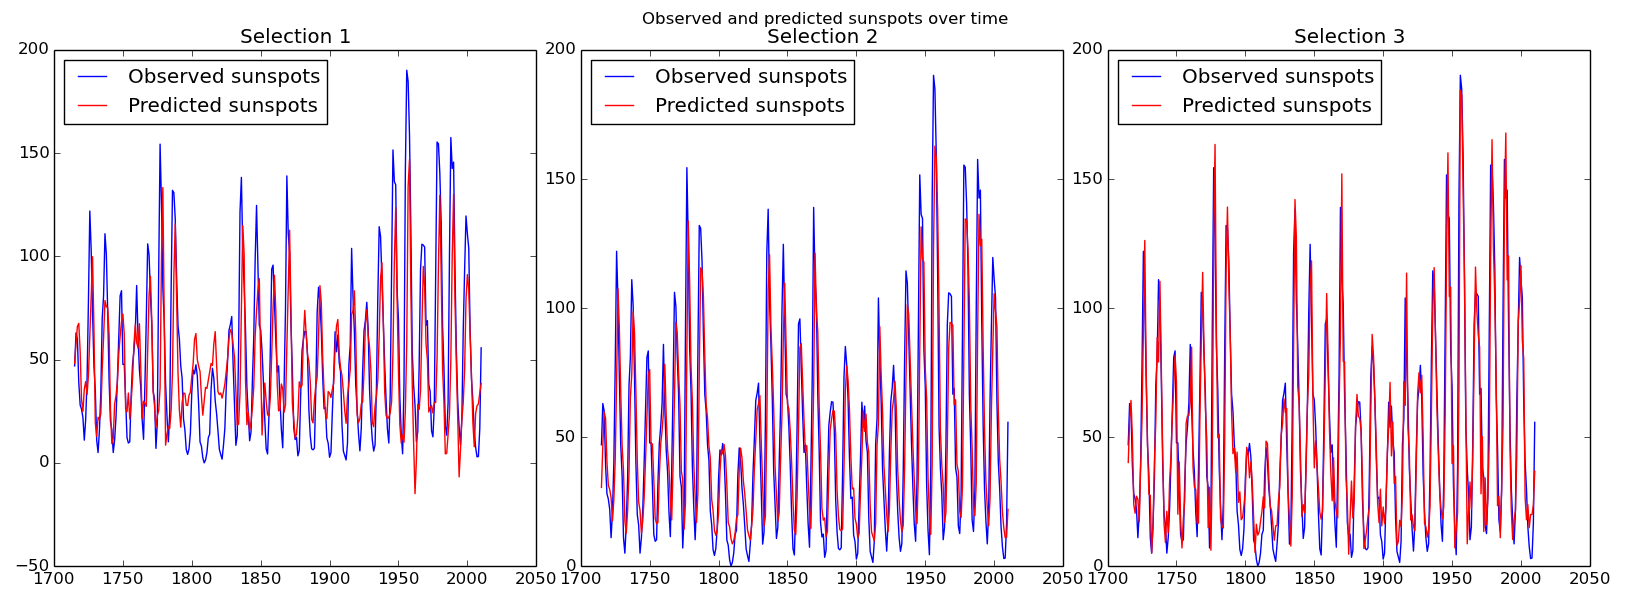
\includegraphics[width=\textwidth]{src/img/obs_over_time}
    \caption{Showing how the different selections fit with acutal observations. We see all models account for the recurring ups and downs, but only selection 3 matches all hills and valleys well.}
    \label{fig:obs_time}
\end{figure}

\subsection{II.2.2 Maximum a posteriori solution}

Done, see \texttt{src/II.2.2.py}.\\

The plots are:\\

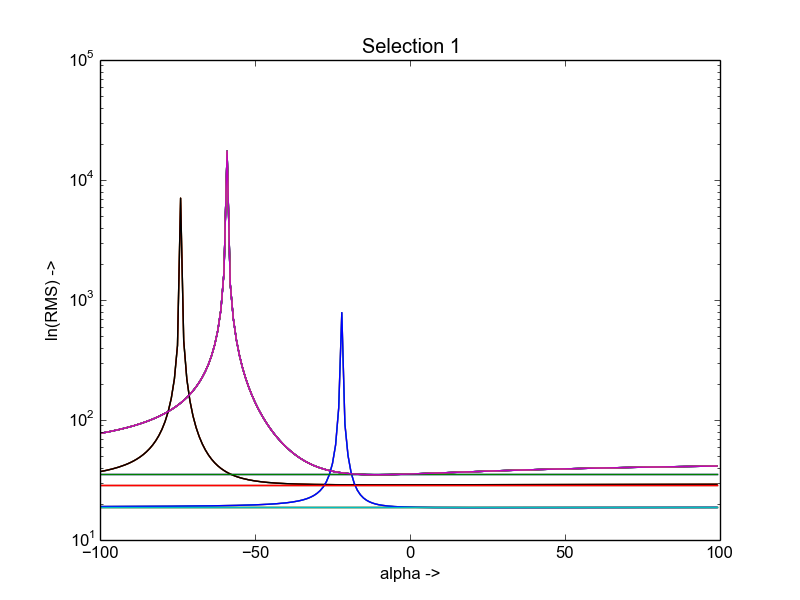
\includegraphics[keepaspectratio=true, width=350pt]{src/img/sel1.png}

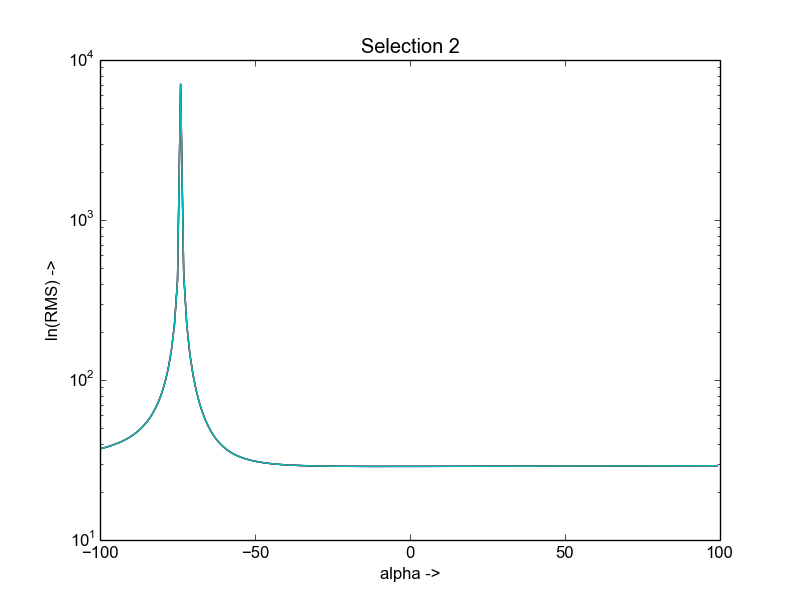
\includegraphics[keepaspectratio=true, width=350pt]{src/img/sel2.png}

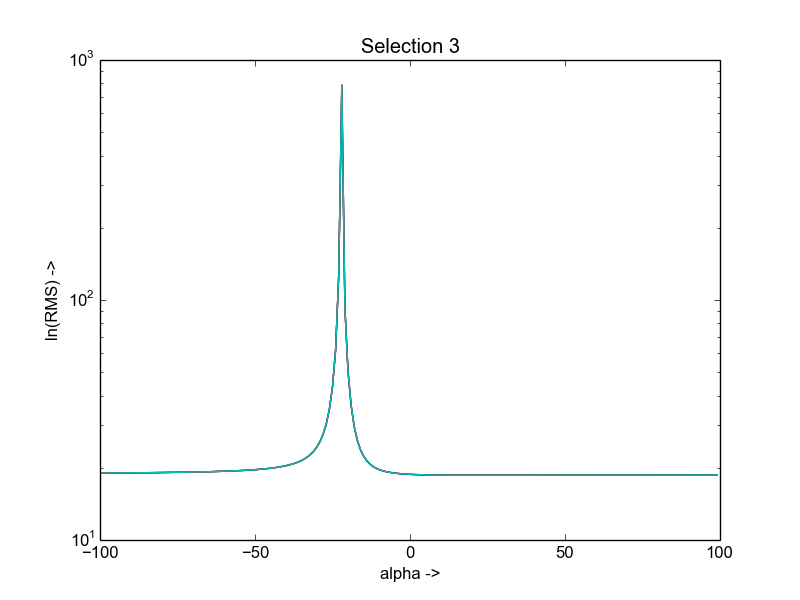
\includegraphics[keepaspectratio=true, width=350pt]{src/img/sel3.png}

and combined, along with the RMS of the ML results:\\

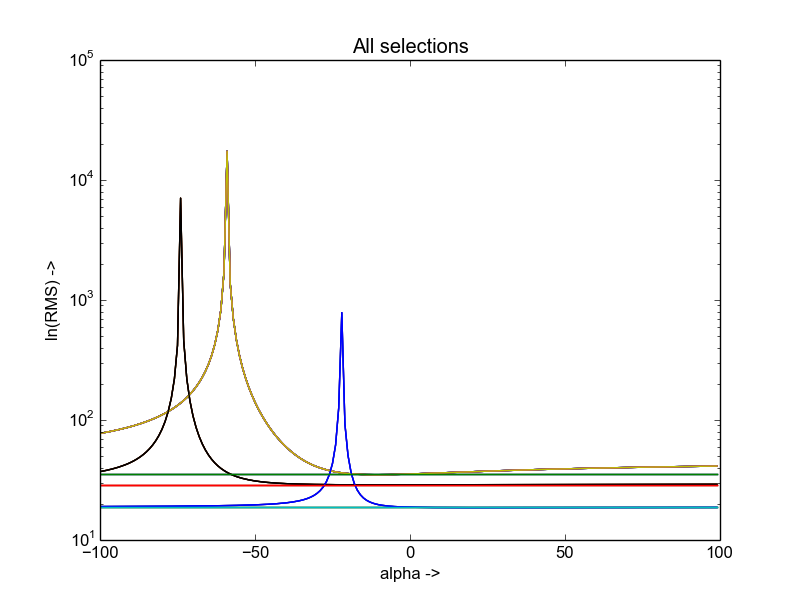
\includegraphics[keepaspectratio=true, width=350pt]{src/img/selall.png}

It seems clear that selection 3 provides the best prediction, and selection 1 the worst. The ML solution scores slightly worse for a narrow range of alpha (-11 for Selection 1, -8 for Selection 2 and 22 for Selection 3), but much better for most choices of alpha.


\subsection{II.2.3 Weighted sum-of-squares (based on CB Ex. 3.3)}

$E_D(\mathbf{w})=\frac{1}{2}\sum_{n=1}^Nr_n\{t_n-\mathbf{w}^T\mathbf{\phi}(\mathbf{x}_n)\}^2$\\

To find the minimum we solve $\frac{\delta}{\delta w_i}E_D=0$ for all $i$:\\

$\frac{\delta}{\delta w_i}E_D=\sum_{n=1}^Nr_n(t_n-\mathbf{w}^T\mathbf{\phi}(\mathbf{x}_n))\cdot(-\phi_i(\mathbf{x}_n))=0$ for all $i$\\

Since $\mathbf{\phi}(\mathbf{x})^T=(\mathbf{\phi}_0(\mathbf{x}),\mathbf{\phi}_1(\mathbf{x}),\dots,\mathbf{\phi}_{n-1}(\mathbf{x}))$, we get\\

$\sum_{n=1}^Nr_n\mathbf{w}^T\mathbf{\phi}(\mathbf{x}_n)\mathbf{\phi}(\mathbf{x}_n)^T-\sum_{n=1}^Nr_nt_n\mathbf{\phi}(\mathbf{x}_n)^T=0$\\

or\\

$0=\mathbf{w}^T\sum_{n=1}^Nr_n\mathbf{\phi}(\mathbf{x}_n)\mathbf{\phi}(\mathbf{x}_n)^T-\sum_{n=1}^N(r_nt_n\mathbf{\phi}(\mathbf{x}_n)^T)$ (*)\\

Setting $\Phi=\left(\begin{matrix}\mathbf{\phi}_0(\mathbf{x}_1) & \mathbf{\phi}_1(\mathbf{x}_1) & \dots & \mathbf{\phi}_{M-1}(\mathbf{x}_1) \\
\vdots & & & \vdots \\
\mathbf{\phi}_0(\mathbf{x}_N) & \mathbf{\phi}_1(\mathbf{x}_N) & \dots & \mathbf{\phi}_{M-1}(\mathbf{x}_N)\end{matrix}\right)$ we rewrite (*) as\\

$0=\mathbf{w}^T(\mathbf{\Phi}^T\mathbf{r}\mathbf{\Phi})-\mathbf{r}\mathbf{t}^T\mathbf{\Phi}$\\

$\Rightarrow\mathbf{w}^T(\mathbf{\Phi}^T\mathbf{r}\mathbf{\Phi})=\mathbf{r}\mathbf{t}^T\mathbf{\Phi}$\\

$\Rightarrow(\mathbf{\Phi}^T\mathbf{r}\mathbf{\Phi})^T\mathbf{w}=(\mathbf{\Phi}^T\mathbf{r}\mathbf{\Phi})\mathbf{w}=\mathbf{\Phi}^T\mathbf{r}\mathbf{t}$\\

$\Rightarrow\mathbf{w}^*=(\mathbf{\Phi}^T\mathbf{r}\mathbf{\Phi})^{-1}\mathbf{\Phi}^T\mathbf{r}\mathbf{t}$\\

\subsubsection{Data dependent noise variance}

If a data point is far from the expected value, the weighting can be used to give that point less importance when minimizing the error.

\subsubsection{Replicated data points}

Replicated data points will usually hold undue importance, but the weights can be chosen lower for the replicated points to counter this.

%% \newpage

%% Since $\mathbf{\phi}(\mathbf{x})^T=(\mathbf{\phi}_0(\mathbf{x}),\mathbf{\phi}_1(\mathbf{x}),\dots,\mathbf{\phi}_{n-1}(\mathbf{x}))$, we get\\

%% $\sum_{n=1}^Nr_nt_n\mathbf{\phi}(\mathbf{x}_n)^T-\sum_{n=1}^Nr_n\mathbf{w}^T\mathbf{\phi}(\mathbf{x}_n)\mathbf{\phi}(\mathbf{x}_n)^T=0$, so\\

%% $\sum_{n=1}^Nr_nt_n\mathbf{\phi}(\mathbf{x}_n)^T-\mathbf{w}^T\sum_{n=1}^Nr_n\mathbf{\phi}(\mathbf{x}_n)\mathbf{\phi}(\mathbf{x}_n)^T=0$\\

%% Setting $\Phi=\left(\begin{matrix}\mathbf{\phi}_0(\mathbf{x}_1) & \mathbf{\phi}_1(\mathbf{x}_1) & \dots & \mathbf{\phi}_{M-1}(\mathbf{x}_1) \\
%% \vdots & & & \vdots \\
%% \mathbf{\phi}_0(\mathbf{x}_N) & \mathbf{\phi}_1(\mathbf{x}_N) & \dots & \mathbf{\phi}_{M-1}(\mathbf{x}_N)\end{matrix}\right)$ we rewrite as\\

%% $((\mathbf{I}\mathbf{r})\mathbf{t})^T\mathbf{\Phi}-\mathbf{w}^T(\mathbf{\Phi}^T\mathbf{r}\mathbf{\Phi})=0$, or\\

%% $\mathbf{w}^T(\mathbf{\Phi}^T\mathbf{r}\mathbf{\Phi})=((\mathbf{I}\mathbf{r})\mathbf{t})^T\mathbf{\Phi}$, so\\

%% $(\mathbf{\Phi}^T\mathbf{r}\mathbf{\Phi})\mathbf{w}=((\mathbf{I}\mathbf{r})\mathbf{t})^T\mathbf{\Phi}$, thus\\

%% $\mathbf{w}^*=(\mathbf{\Phi}^T\mathbf{r}\mathbf{\Phi})^{-1}((\mathbf{I}\mathbf{r})\mathbf{t})^T\mathbf{\Phi}$, and\\

%% $\mathbf{w}^*=$

% \includegraphics[keepaspectratio=true, width=350pt]{src/img/II_2_3-1.jpg}

% \includegraphics[keepaspectratio=true, width=350pt]{src/img/II_2_3-2.jpg}






\end{document}
